\section{Standard Model W$\gamma$ Production}
\label{sec:WgAbout_SMproduction}

A $W$ boson in proton-proton collisions can be produced in the processes $q {\bar{q'}} \rightarrow W$ where $q$ and $\bar{q'}$ are a quark and an antiquark which have a total charge of $+1$ if producing a $W^+$ boson or $-1$ if producing a $W^-$ boson. The processes $u\bar{d}\rightarrow W^+$ and $d\bar{u}\rightarrow W^-$ are the most likely to occur because $u$ and $d$ are valence quarks in a proton. There are twice as many $u$ quarks in a proton as $d$ quarks, therefore, $W^+$ is produced twice more frequently than $W^-$. Antiquarks $\bar{d}$ and $\bar{u}$ come from the sea $q\bar{q}$ pairs of the other proton.\\

Once created, a $W$ boson decays immediatelyi, its lifetime is~$\simeq 10^{-25}$~s. In an experiment one detects its decay products rather than the $W$ boson itself. Decay modes of a $W$ boson include $W^\pm \rightarrow l^\pm \nu_l ({\bar{\nu_l}})$ where $l^\pm=e^\pm$, $\mu^\pm$ or $\tau^\pm$ with branching fractions of ~11\% per a leptonic channel \cite{ref_PDG}. The remaining 67\% account for various $W\rightarrow q\bar{q'}$ decays. In this dissertation we only consider $W^\pm \rightarrow \mu^\pm \nu_\mu ({\bar{\nu_\mu}})$ and $W^\pm \rightarrow e^\pm \nu_e ({\bar{\nu_e}})$ channels.\\

% MAY NOT NEED THIS
%Mass of a $W$ boson $M_W=80$ GeV is much larger than masses of its decay products: $M_\mu=105$ MeV, $M_e=0.5$ MeV, $M_\nu<2$ eV. Therefore, almost all mass of a $W$ boson converts to the kinetic energy of the muon or electron and neutrino or antineutrino.\\

A photon can be emitted from any charged particle of the process: a quark, an antiquark, a charged lepton or a $W$ boson (Fig.~\ref{fig:feynmWg_LO_NLO}, top). A quark and an antiquark are initial state particles and, therefore, if one of them radiates a photon, we refer to the process as initial state radiation (ISR). A muon or an electron is a final state particle and if it radiates a photon, we call such a process final state radiation (FSR). Finally, a $W$ boson is a gauge boson and if it radiates a photon, the process has a vertex with three gauge bosons: $WW\gamma$, and we call such process the triple gauge coupling (TGC). We cannot distinguish between these processes experimentally because we detect final state particles only.\\

\begin{figure}[htb]
  \begin{center}
    {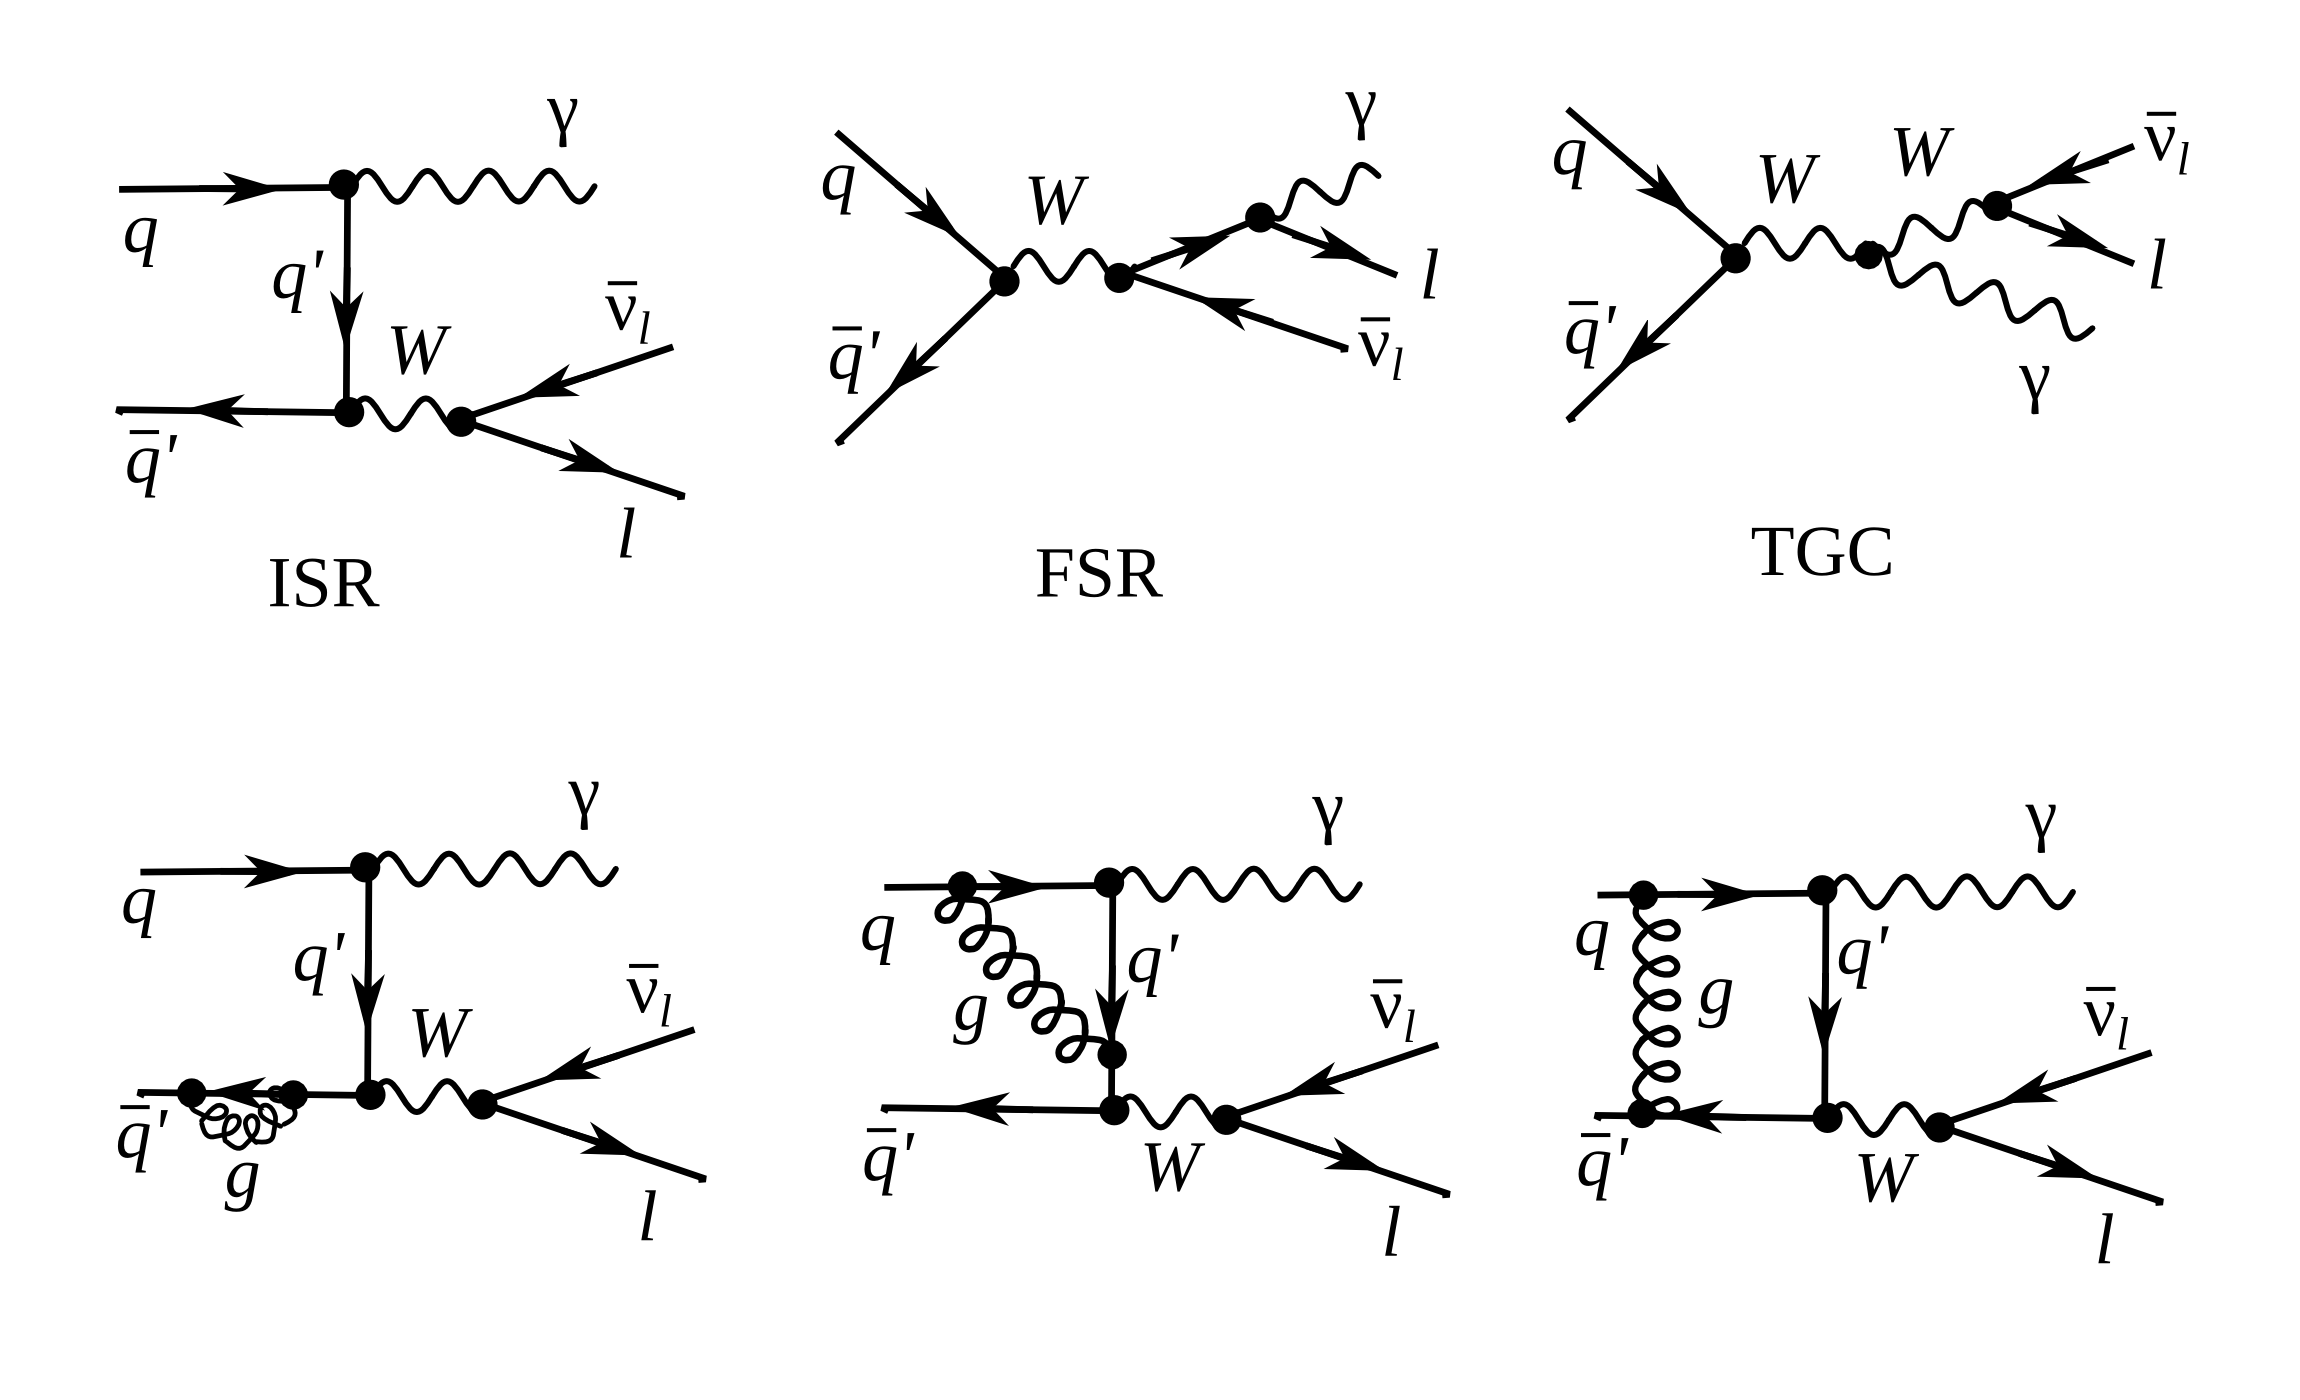
\includegraphics[width=0.90\textwidth]{../figs/WgAbout/feynmWg_LO_NLO.png}}
    \caption{Feynman diagrams of W$\gamma$ production. Top: LO diagrams, bottom: several examples of NLO in QCD.}
    \label{fig:feynmWg_LO_NLO}
  \end{center}
\end{figure}

The electroweak Lagrangian is described in Chapter~\ref{sec:WgAbout_SMEWK}. It is possible to derive equations of motion from the Lagrangian for any fields involved~\cite{ref_Griffiths}. However, in a quantum field theory equations of motion cannot be solved exactly and, therefore, the perturbative approach is used if a coupling constants is $g \ll 1$.\\

To represent the process graphically Feynman diagrams were invented. Also the diagrams can be used to calculate the process amplitude $M$ in Eq.~\ref{eq:FermiGoldenRule} because they are determined by Lagrangian terms relevant to the process. There are an infinite number of Feynman diagrams corresponding to any specific process and the total amplitude of the process is a sum of individual amplitudes of each diagram and it is not technically possible to take into account all of them. Each vertex introduces a factor in the amplitude of the process that is proportional to the coupling constant. If the coupling constant is $g \ll 1$, the perturbative approach arranges all the diagrams by orders of contribution, and, therefore, the Feynman diagrams with fewer vertices would give a significantly larger contribution to the amplitude. In Fig.~\ref{fig:feynmWg_LO_NLO} examples of the Leading Order (LO) and the Next-to-Leading Order (NLO) Feynman diagrams are shown (top and bottom diagrams respectively).\\

At LO, the W$\gamma$ process is represented by four Feynman diagrams including one FSR, one TGC and two ISR diagrams. Each LO diagram has three vertices. The first calculation of the W$\gamma$ process with necessary expressions can be found in~\cite{ref_theory_LO}.\\

The NLO corrections to the amplitude of the $W\gamma$ process that are shown in Fig.~\ref{fig:feynmWg_LO_NLO} are QCD corrections only, which include gluon loops at the same quark line and exchange of a gluon between two different quark lines, however, QED and weak NLO diagrams are also possible. QED corrections involve radiations of extra photons by charged particles, exchange of photons between different charged particles or a photon can be radiated and absorbed by the same charged particle forming a loop. Similarly, weak corrections involve extra virtual $W$ or $Z$ bosons. The QCD corrections are the largest among the discussed correction types because the QCD coupling constant is the largest.\\

A theoretical cross section in particle physics is compared to a measurement result to test the predictions of the model. Also the theoretical cross section is used for producing simulated data. In a simulation, a large set of $pp$ collisions resulting in a physics process of interest is modeled to create a data set that mimics real data. A typical simulation consists of two parts: the generation of the process and the simulation of particles paths through the detector. The first stage contains a collection of events with final state particles with kinematic quantities distributed according to theoretical predictions for a given process. This stage relies on the theory including the cross section and also all dynamics of the process. The second stage simulates the interaction with media during propagation of particles through the model of the detector as well as the response of detector electronics. In its final form, a simulated dataset has the same format and content of detector signals for each event as real data, and can undergo the same reconstruction and analysis procedure as real data would.\\

The most precise theoretical $W\gamma$ cross section available is the Next-to-Next-to-Leading Order (NNLO) cross section in QCD~\cite{ref_theory_NNLO}. The effects of the NNLO correction over the NLO correction and over the LO result are shown in Fig.~\ref{fig:Theory_NNLO_and_other} for the transverse mass of the final state particles $m_T^{l \nu \gamma}$ and for the rapidity difference between a charged lepton and a photon $\Delta_{l\gamma}$. The NNLO and NLO theoretical predictions for the photon transverse momentum $p_T^\gamma$ are overlaid with the~7~TeV ATLAS result. The contribution from higher order corrections is estimated to be $\pm$4\%. However, the NNLO theoretical result was published only recently, in 2015, and no NNLO $W\gamma$ simulation is available at this time. The simulation used in this analysis is LO + up to two hadronic jets simulation which was found to give the same predictions as the NLO result.\\
% [REFERENCE to APPENDIX?].\\

\begin{figure}[htb]
  \begin{center}
    {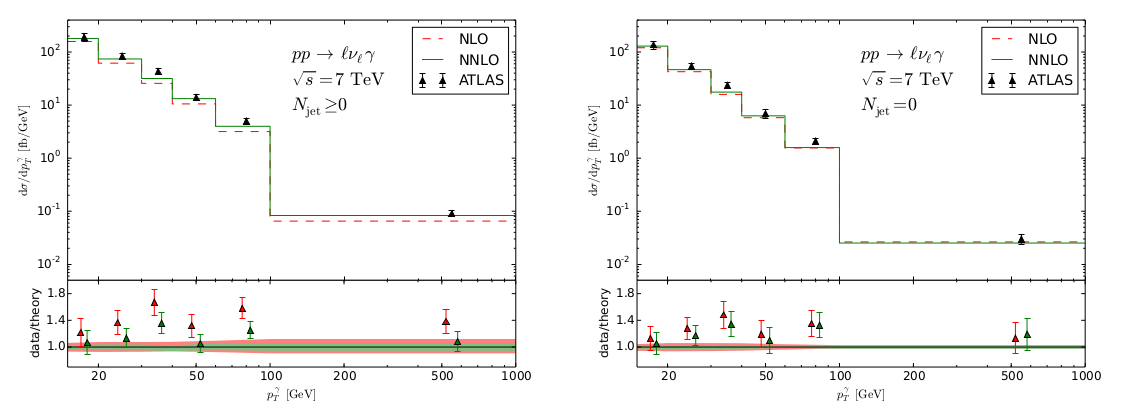
\includegraphics[width=0.95\textwidth]{../figs/WgAbout/Theory_NNLO_PtGamma.png}}    
    {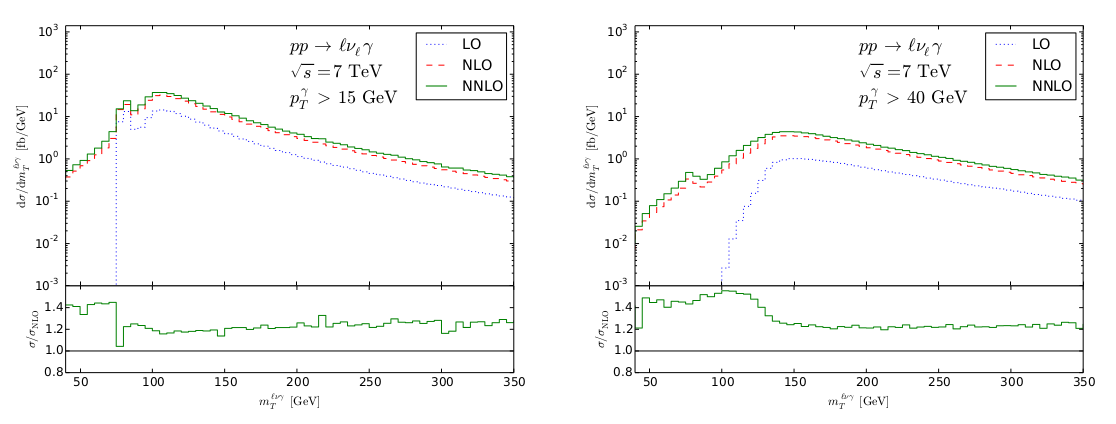
\includegraphics[width=0.95\textwidth]{../figs/WgAbout/Theory_NNLO_mT_finer.png}}
    {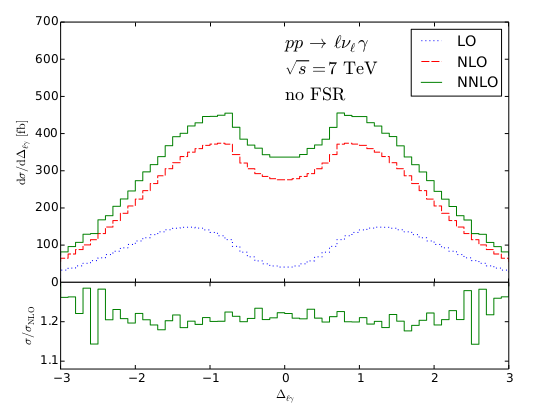
\includegraphics[width=0.50\textwidth]{../figs/WgAbout/Theory_NNLO_rapidity.png}}
    \caption{Theory spectra. Top: NLO and NNLO $p_T^\gamma$ spectra of $W\gamma\rightarrow l\nu\gamma$ at $\sqrt{s}=7$~TeV overlaid with ATLAS data for $N_{jet} \geq 0$ (left) and $N_{jet}=0$ (right). Middle: LO, NLO and NNLO $m_T^{l\nu\gamma}$ spectra of $W\gamma\rightarrow l\nu\gamma$ at $\sqrt{s}=7$~TeV for $P_T^\gamma>15$~GeV (left) and $P_T^\gamma>40$~GeV (right). Bottom: LO, NLO and NNLO $\Delta_{l\gamma}$ spectra of $W\gamma\rightarrow l\nu\gamma$ at $\sqrt{s}=7$~TeV.}
    \label{fig:Theory_NNLO_and_other}
  \end{center}
\end{figure}

Certain BSM theories predict an enhancement of the contribution from the TGC diagram over the SM prediction. The discussion of these BSM effects and how they affect the $W\gamma$ process takes place in Ch.~\ref{sec:WgAbout_ATGC}.\\ 

